\documentclass[11pt,a4paper]{article}
\usepackage[utf8]{inputenc}
\usepackage{amsmath}
\usepackage{amsfonts}
\usepackage{amssymb}
\usepackage{graphicx}

\usepackage{pdfpages}
\usepackage[english]{babel}
\usepackage[hidelinks]{hyperref}
\usepackage[backend=biber]{biblatex}
\bibliography{bib}

\author{Leo Touroul and Charles Bine}
\title{Structured compression}
\date{December 20, 2016}
\begin{document}

	\maketitle

	\section{Why structured compression?}
	
	
	
	Classifying datasets is an active field of research that allows to develop new technology mainly in image and sound recognition.
	The bottleneck when trying to classify datasets are the matrix multiplications happening in the neural networks used to classify the data.
	In order to tackle this bottleneck, and thus allow to run classifying models more rapidly, or at the same speed with cheaper/smaller components, one can use the concept of dimensionality reduction.
	
	Decreasing the dimensionality of the dataset being learned results in reducing the number of basic operations computed by the hardware during the matrix multiplications and therefore speed up the classification.
	However, there is a limit to the number of dimensions we can reduce the dataset we want to classify to. This paper will delve into the concept of dimensionality reduction using structured compressions.
	
	Indeed, matrix multiplication for matrices of size $n*n$ is an operation requiring $O(n^3)$ time complexity. Moreover, matrix multiplication are the basic operations in machine learning, when using the basic feed forward structure in the back propagation algorithm. Reducing the dimensionality of the problem therefore has a dramatic speedup on the run time.
	
	
	

	
	\section{Setup experimental setup}
	
	To study the effect of dimensionality reduction using structured compression, we are going to use the classic MNIST dataset of handwritten digits. This dataset consists in grey-scale $28 \times 28$ images representing digits. Each image is associated with a label describing the digit represented by the image. Figure \ref{img:example_mnist_img} shows what an image from the dataset might look like. In that case, the associated label is "7". 
	
	This image is just a matrix of size 28 by 28. Each cell of the matrix represents a pixel. The value in each cell is an int between 0 and 256 representing a shade of grey.
	
		\begin{figure}
			\centering
			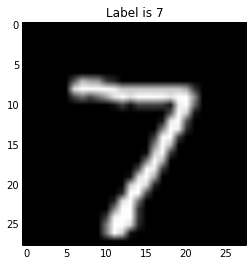
\includegraphics[scale=0.7]{img/gYsJp.png}
			\caption{An example image from the MNIST dataset. In this case, the label is "7".}
			\label{img:example_mnist_img}
		\end{figure}
		
	
	This dataset can be found at \url{http://yann.lecun.com/exdb/mnist/}. It is de facto split in 2 subsets : a training set (60k entries) and a test set (10k entries). We will devide the training set into 50k entries of training and 10k for validation. We decided to run our study on the dataset resulting of the merge of the training set and the dataset.
	

	When we want to classify a dataset, we have to separate it in a training set and a test set. The training set is used to train the classifier (usually a neural network), and the test set is used to verify that the classification is working for general inputs, and is not over-fitted to the training set. You can see this as making sure that the classifier didn't learn by heart the inputs contained in the training set.
	Here, we merged the training set and test set to then be able to choose the number of images used in the training set and the testing set. Merging and splitting them as we wish allows us to have different proportion of input data in the training set and the test set.
	
	The programming language used in this study is Python 3.5, allowing us to plug in powerful mathematical, statistical and plotting tools, on top of the new machine learning framework Tensorflow.
	This framework is a useful interface when we want to easily run the computations on GPU, which provides a huge speed up compared to running the computations on CPU because it is highly optimized for massively parallelisable operations, such as computing matrix products. 
	
	\subsection{Structured compression}
	Before we speak about structured compression, let's speak about classic compression. A compression part is just used to decrease the dimensionality of the input data (in the case of the MNIST dataset, each image is in the $[0, \dots, 256]^{28*28}$ space as we can consider a 28 by 28 matrix as a flat vector of size 28*28). Compressing the MNIST dataset means finding a mapping between $\mathbb{R}^n$ to $\mathbb{R}^d$ where n is the dimensionality of the pristine, uncompressed input, and d is a number smaller than n.
	
	
	An easy compression mapping to understand is just the action of dropping components. For example in MNIST, if we decided to naively drop the last 200 hundred components, we would end up in $[0,\dots, 256]^584$, which will allow us to run the learning phase faster due to a reduce number of basic operations in the matrix multiplications.
	
	
	Why is this reduction naive? Because dropping arbitrarily the last 200 components might lead to the loss of important information. A better classic compression will take into consideration all the original components of the input data (all the pixels in the case of image recognition with MNIST), such that we don't lose any information.
	
	
	There drop mapping could be seen as a simple identity matrix bloc completed by only zeros. This compression leads to a loss of information that won't allow us to classify the dataset in the same way as we would have done on the original dataset.
	
	Before we dive into a better classic compression and structured compression, let's notice that if we want to be able to classify a compressed dataset and obtain almost the same results as when we classify the uncompressed dataset, we need an invariant. Something that will allow us to say that two inputs in the same class/set/group are close together, and that two inputs that are in different classes/sets/groups are far from each other. Each input can be seen as a vector in the $\mathbb{R}^n$ space. After the compression, the same input is a vector in the $\mathbb{R}^d$ space. What comes to mind as an invariant would be a distance, a notion that expresses clearly the fact that two inputs are similar when they are close to each other, and different when they are far from each other.
	
	
	Note that we don't know yet which distance to use. However, since we are working in finite dimension, all the norms are equivalent, and it is therefore convenient and not restricting to chose the Euclidean distance ($L^2$ norm), as one possible distance. Another distance that could be chosen is the angular distance.
	
	A great compression is therefore a compression that won't change a given distance by much. There's a theoretical limit to the level of compression we can achieve, if we want to keep the accuracy within a certain range, and this theoretical result is given by the JLT theorem.
	
	
	\paragraph{Johnson–Lindenstrauss lemma}
	Given $0 < \varepsilon < 1$, a set $X$ of $m$ points in $\mathbb{R}^N$, and a number $n > \frac{8 \ln(m)}{\varepsilon^2}$, there is a linear map $f : \mathbb{R}^N \mapsto \mathbb{R}^n$ such that:
	
	\begin{equation}
		\forall u,v \in X \quad (1-\varepsilon)\|u-v\|^2 \leq \|f(u) - f(v)\|^2 \leq (1+\varepsilon)\|u-v\|^2
	\end{equation}
	

	We can demonstrate that $\frac{G}{\sqrt(d)}$ where each coefficient of $G$ is either picked independently into $N(0,1)$ a standard Gaussian random variable, or $\{-1,1\}$ (mean 0, variance not 0) will compress the dataset to $R^d$ (G is of size $\mathbb{R}^n,d$) and will keep the Euclidean distance between two compressed inputs close to the original euclidean distance between the two uncompressed inputs.
	
	***Here is the proof, if you don't have it I'll send a picture, it's quite fast***
	
	This compression is a great tool that will allow us to run the learning phase faster. However, this compression is a matrix multiplication of overall time complexity $O(dnp)$, where $d$ is the target dimension of the compression, $n$ the original dimension, and $p$ the number of inputs.  
	
	This is resource consuming, and we can speed up this phase using structured compression:
	
	The idea behind structured compression is that instead of using a $n*d$ matrix, we can use build up a $n*d$ matrix repeating some components. When done in a clever way, both the spatial complexity and the time complexity can be decreased.
	
	The first building block of structured compression is a circulant matrix, let's call it $G_{circ}$. Instead of compressing the input dataset by multiplying it by $\frac{G}{\sqrt(d)}$, we can reduce it using a $\frac{G_{circ}}{\sqrt(d)}$ multiplication. Instead of storing $n \times d$ independent stochastic components, we just store n of them and the matrix is built shifting those components by one at every row: 
	
	\begin{equation*}
        G_{circ}=
        \begin{bmatrix}
        g_0     & g_{n-1} & \dots  & g_{2} & g_{1}  \\
        g_{1} & g_0    & g_{n-1} &         & g_{2}  \\
        \vdots  & g_{1}& g_0    & \ddots  & \vdots   \\
        g_{n-2}  &        & \ddots & \ddots  & g_{n-1}   \\
        g_{n-1}  & g_{n-2} & \dots  & g_{1} & g_0 \\
        \end{bmatrix}.
	\end{equation*}

	
	
	What is also great with this matrix, on top of the fact that the space required to store it is reduced, is that the time to compute $G_{circ} \times Data$ (where $Data$ is the input) can be reduced to $n*log(d)$ using Fast Fourier Transform (FFT).
	 
	 
	However, reducing the number of non deterministic parameters leads to a loss of independence of the coefficient. We can't split the expectation as seen in the previous proof saying that $g_{i,j_1} g_{i,j_2}$ are independent. To retrieve this independence property, we can multiply this circulant matrix with a diagonal matrix where the coefficients are chosen independently from a $N(0,1)$ or $\{-1,1\}$ with equip-probable outcomes.
	
	Another key idea in those structured compression is that we need balance before we compress the data, we need to spread the data points evenly across all the space to make sure we are not compressing packed data. A way to achieve balance is to use Hadamard matrices.
	
	
	
	
	Thanks to the properties of a Hadamard matrix, we can compute the matrix multiplication with an input vector in $O(n*log(n))$ if $n$ is a power of $2$.
	
	
	\[
	H_1 = \begin{bmatrix}
		1      \end{bmatrix},
	\]
	
	\[
	H_2 = \begin{bmatrix}
		1 &  1 \\
		1 & -1 \end{bmatrix},
	\]
	
	and
	
	\[
	H_{2^k} = \begin{bmatrix}
		H_{2^{k-1}} &  H_{2^{k-1}}\\
		H_{2^{k-1}}  & -H_{2^{k-1}}\end{bmatrix} = H_2\otimes H_{2^{k-1}},
	\]
	
	for $ 2 \le k \in N $, where $ \left.\otimes\right. $ denotes the Kronecker product.
	
	
	
	To sum up, the two main parts of structured compression are:
	\begin{enumerate}
		\item Balance the data using a rotation matrix. The Hadamard matrix, thanks to it's recursive definition allows us to compute this step with small space complexity and in $O(nlog(n))$ time.
		\item Compress the data using a projection matrix. Here we can use a G matrix, or as proved just above, we can use a $G_{circ}$ matrix to speed up the computation ($O(nlog(d))$ achieved) and reduce the space complexity. To maintain the independence characteristic, we just need to use a diagonal matrix before we compute the compression using FFT.
	\end{enumerate}

	

	
	
	
	\section{Results}
	
	
	Let's consider 2 datasets, one is the original one, let's call it \texttt{dataset\_original}, the second one is transformed.
	
		A transformation in our study is defined by a matrix multiplication to provide a structured compression (for sure, the structured compression is equivalent to a matrix multiplication, but to benefit the speed ups of structured compressions, we implemented the structured compression using FFT, and Hadamard specificity mainly using python scipy package), and a function applied element-wise. Therefore, a transformation is defined by 3 parameters, a matrix (representing the structured compression) used for the reduction, a target dimension, and a function.
		
		
	The notation \texttt{d\_m\_td\_f} represents the dataset where the matrix m with target dimension td and function f were applied.
	
	Let's consider a transformed dataset. The idea is that we are going to take a set of 2uples representing 2 images. For each 2uple, we are going to compute the distance (which one is to be determined) between those two points:
	
	\begin{enumerate}
		\item picked from the original, not transformed dataset,
		\item picked from the transformed data set
	\end{enumerate}


	
	
	Then we divide the second distance by the first distance. As explained before, if the distance is conserved when we apply a compression, we should be able to classify the data with the transformed dataset as good as with the original dataset, but faster. We suppose this is true with the euclidean distance, meaning that if the distances between two random points in the transformed dataset is roughly similar to the distance between the two original points in the original dataset, we won't have any problem classifying the data using the transformed dataset.
	
	
	Therefore, if we compute a huge number a quotient of distances, and we plot those results, we should expect a Gaussian with mean 1 and small variance for a transformation that keeps the properties of the original dataset and then allows us to classify it.
	
	The various transformations can be found in the annex \ref{graphs} of this document.
	
	
%	\includepdf[nup=2x4, pages={33-52}, delta = 20 20]{img/all.pdf}
	
%	\begin{figure}
%		\centering
%		\begin{minipage}{.5\textwidth}
%			\centering
%			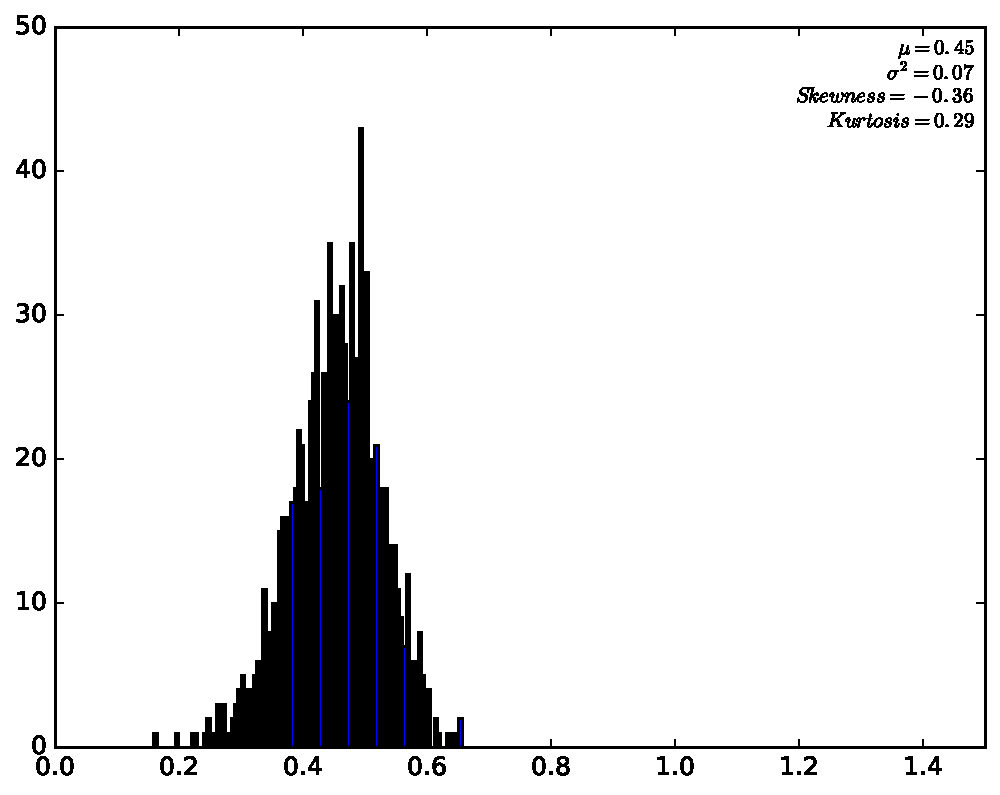
\includegraphics[width=.8\linewidth]{img/t_Drop_d_256_f_Identity.pdf}
%			\caption{t\_Drop\_d\_256\_f\_Identity}
%		\end{minipage}%
%		\begin{minipage}{.5\textwidth}
%			\centering
%			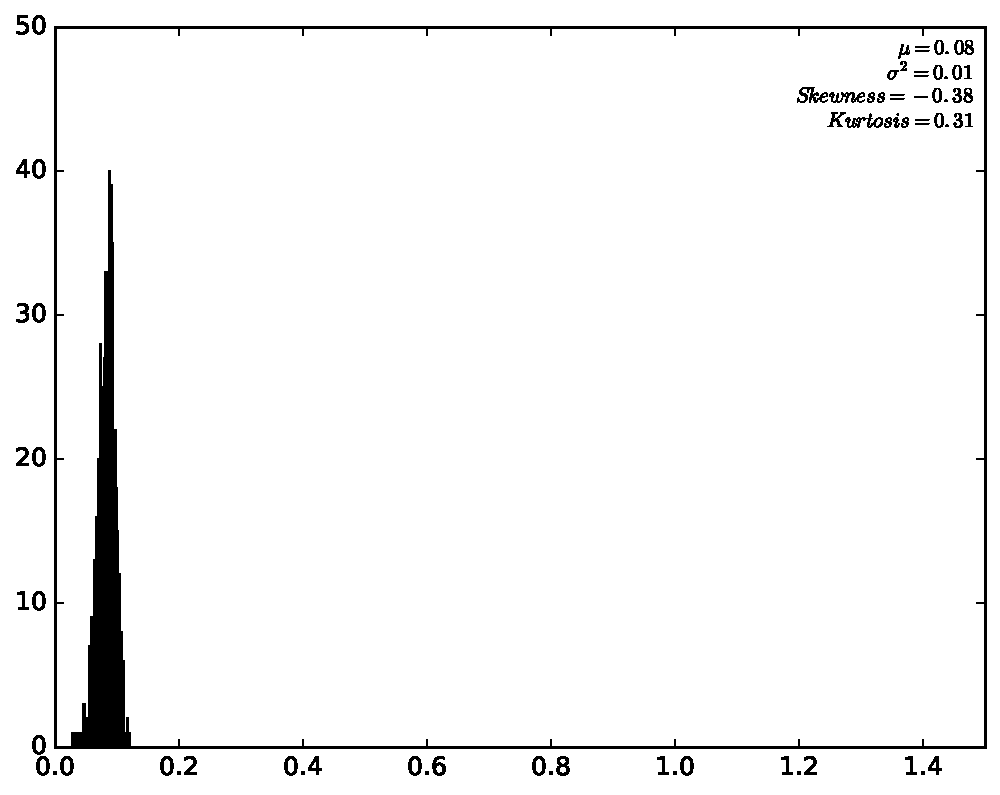
\includegraphics[width=0.8 \linewidth]{img/t_Drop_d_256_f_Sigmoid_diff.pdf}
%			\caption{t\_Drop\_d\_256\_f\_Sigmoid diff}
%			\label{fig:test2}
%		\end{minipage}
%	\end{figure}
%	

	As we can see with the graphs, we can reduce the dimension a significant amount without loosing much information regarding the euclidean distance. When the quotient of distance when we apply a function is not 1, we would have to improve the nonlinear element-wise function and better tune them to get better results. 
	
	
	\section{Classify}
	
	We used the framework Tensorflow for the classification part. This framework provides useful neural networks out of the box with little need to be tuned and adapted. We first set up a simple softmax neural network to get familier with tensorflow's tensors and syntax. This feed forward neural network containing 1 hidden layer yields around 90\% of accuracy and runs in less than a second on CPU to classify MNIST pristine dataset.
	
	
	We then implemented a convolutional neural network with 2 feature maps layers, 2 pooling layers, and adding some drop out. This architecture yielded an satisfying 99.2\% of accuracy on MNIST pristine dataset but it took 30min of CPU time to train the model. On GPU, the computation time is expected to be a lot smaller but we unfortunately did not have access to a GPU compatible with cudNN (compute capability of 3.1 or 5.2)
	
	
	We therefore decided to run the classification using softmax feed forward neural networks. We were not able to run days of computation to get better accuracies using the second architecture. We still ran the second architecture on some transformed dataset to check if the speed up were working, and the accuracy wasn't lowered a lot. 
	
	
	Here are the results of the classification of the MNIST dataset, going through various pipelines, using a basic softmax feed forward neural network containing 1 hidden layer, with a learning rate of 0.5 and batch size of 100:
	
	
	\paragraph{Pipeline}
	\begin{itemize}
			\item Transform: Identity
			\item Target dimension: 784
			\item Function: Identity
	\end{itemize}
	 \paragraph{Result}
	 \begin{itemize}
			\item Accuracy: 90.7\%
			\item Computation time: 1.xxx s
	\end{itemize}



	
	
	\section{Problems Future improvements}
	The first obvious problem in this study is the lack of GPU access.
	
	
	An improvement, which we will implement as soon as we have access to a GPU with a CUDA compute capability of 5.2, would be to run the classifying part using the second architecture.
	This faster computation pipeline will allow us to run various training phases allowing us to first tune and find the optimal hyperparameters for this dataset.
	
	
	It will also allow us to extend the results to other datasets such as CIFAR-10 and CIFAR-100, which input images are a lot bigger than the one in MNIST, and where the complexity is significantly higher.
	
	
	Being able to run the classification part will allow us to plot the optimal accuracy as a function of the feature map sizes and the stride.
	
	
Once the best parameters are found, we will run the classifying part on all the transformed datasets using various transformation, non linear functions.
	
	Another improvement would be to chain the various transformations and dimensionnality reductions pipelines and compare their efficiencies with those of one unique global dimensionnality reduction pipeline.
	
	
	\section{Conclusion}
This project was a great way to understand in depth the classifying architecture yielding the best result so far in image and sound recognition (convolutional neural networks), and the mechanisms associated with this architecture.

It was also a great way to understand how structured compression works, and how it allows to reduce the computation times, while still preserving the accuracy. This knowledge is important to either run the algorithms linked with artificial intelligence faster, or run them on less efficient pieces of hardware such as mobile phones.


\appendix
\section{Result graphs}
\label{graphs}

On the following page, please find the matrix of transformations. Along the vertical axis, we vary the target dimension. Along the horizontal axis, we vary the transform type.

\vspace*{-8cm}\hspace*{-7cm}
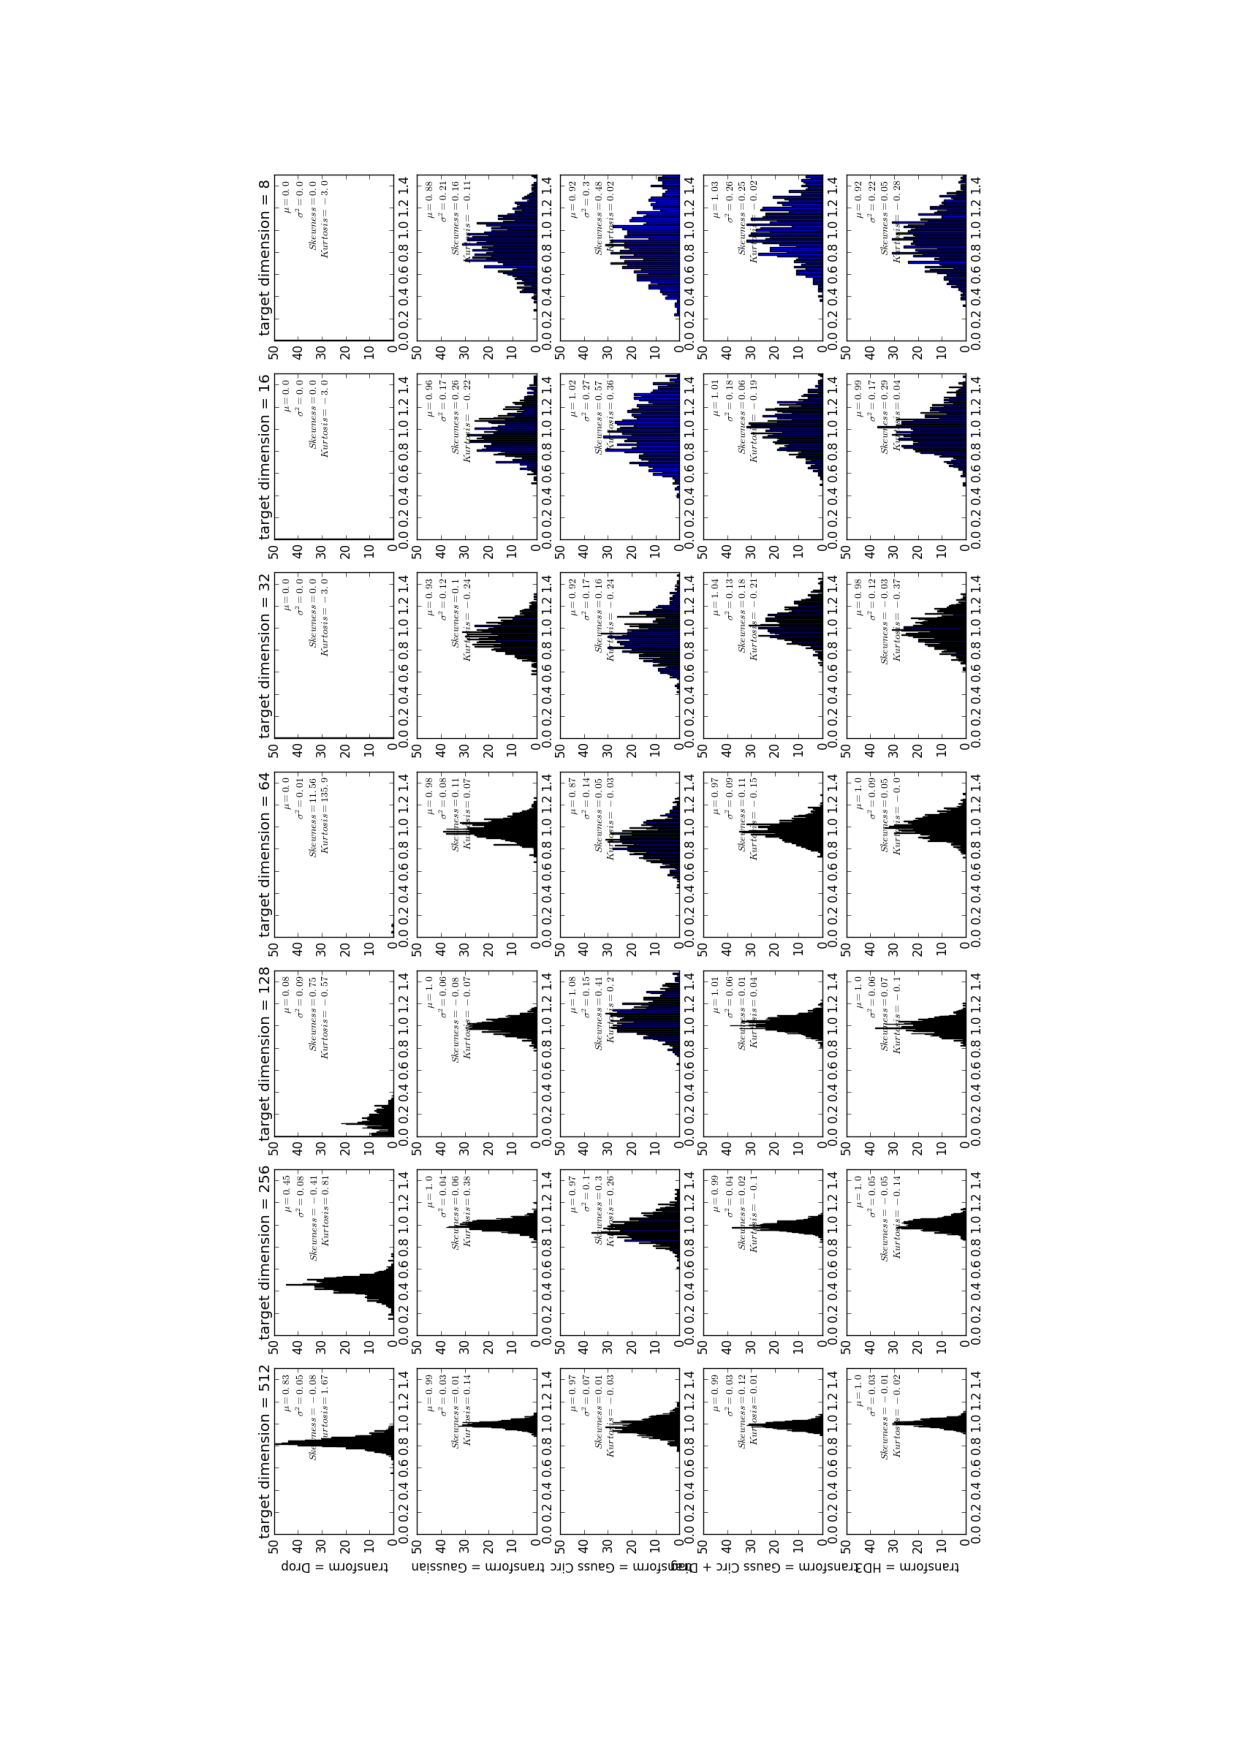
\includegraphics[scale =1.2]{img/annex2.pdf}

	\newpage
	\nocite{*}
	\printbibliography


\end{document}



